\documentclass[twoside, 11pt]{article}

% ------
% Fonts and typesetting settings
\usepackage[sc]{mathpazo}
\usepackage[T1]{fontenc}
\linespread{1.05} % Palatino needs more space between lines
\usepackage{microtype}
\usepackage{lipsum}
\usepackage{tikz}
\usepackage{float}
\usepackage{graphicx}
\usepackage[justification=centering]{caption}
\usepackage{subcaption}

% ------
% Page layout
\usepackage[hmarginratio=1:1,top=32mm,columnsep=20pt]{geometry}
\usepackage[font=it]{caption}
\usepackage{paralist}
\usepackage{multicol}

% ------
% Lettrines
\usepackage{lettrine}

% ------
% Abstract
\usepackage{abstract}
	\renewcommand{\abstractnamefont}{\normalfont\bfseries}
	\renewcommand{\abstracttextfont}{\normalfont\small\itshape}

% ------
% Titling (section/subsection)
\usepackage{titlesec}
\renewcommand\thesection{\arabic{section}}
\titleformat{\section}[block]{\large\scshape\centering}{\thesection.}{1em}{}
\renewcommand\thesubsection{\roman{subsection}}
\titleformat{\subsection}[block]{\normalsize\it}{\thesubsection.}{1em}{}

% ------
% Header/footer
\usepackage{fancyhdr}
	\pagestyle{fancy}
	\fancyhead{}
	\fancyfoot{}
	\fancyhead[C]{Portland State University $\bullet$ December 2015}
	\fancyfoot[RO,LE]{\thepage}

% ------
% Clickable URLs (optional)
\usepackage{hyperref}

% ------
% Maketitle metadata
\title{\vspace{-15mm}%
	\fontsize{24pt}{10pt}\selectfont
	\textbf{Vertical Search Constraints for Multiview Motion Estimation}
	}	
\author{}
\date{}


%%%%%%%%%%%%%%%%%%%%%%%%%%%%%%%%%%%%%%%%%%%%%%%%%%%%%%%%%%%%%%%%%%%%%%%%%%%%%%%%
\begin{document} %%%%%%%%%%%%%%%%%%%%%%%%%%%%%%%%%%%%%%%%%%%%%%%%%%%%%%%%%%%%%%%

\maketitle
\thispagestyle{fancy}

\begin{abstract}
[TODO: add an abstract]
\end{abstract}

\section{Introduction} %%%%%%%%%%%%%%%%%%%%%%%%%%%%%%%%%%%%%%%%%%%%%%%%%%%%%%%%%
\label{sec:introduction} %%%%%%%%%%%%%%%%%%%%%%%%%%%%%%%%%%%%%%%%%%%%%%%%%%%%%%%
Multiview video coding (MVC) is a field that has emerged recently to
enable technologies such as stereoscopic video and free-viewpoint video. In
stereoscopic video, views from different, horizontally separated cameras are
presented to each eye to simulate a 3-dimensional scene. It is frequently useful
to have more than 2 views available to compensate for the viewer's distance from
the screen. Free-viewpoint video uses the views from multiple horizontally
separated cameras to allow the user to choose his vantage point on a scene. In
either case, it is necessary to encode at least two video streams together.

Multiview video presents bandwidth and storage challenges, since it is obviously
more expensive to transport or store multiple viewpoints than it is to transport
or store just one. Fortunately, since all the cameras are focused on the same
scene there is some inter-view redundancy, which can be taken advantage of such
that the combined views can be encoded more efficiently together than they could
be individually.

The mechanism commonly used -- most pertinently, in ITU H.264 and annex H, its
multiview extension -- is block-based motion compensation. This allows some
pictures to be stored with reference to one or two other pictures. Each block
of the dependent view can optionally be stored as a spatial offset, at up to
quarter-pixel resolution, to a similar block in the reference view and a
frequency-domain difference between the dependent and reference blocks.

With this technique, the encoder can reduce inter-view redundancy and save
space, but at the cost of spending time searching the reference pictures for
similar blocks. In general, increasing the search space decreases the resulting
bit-rate, but takes more time. It's reasonable then, to ask what the best
trade-off is between time and efficiency. A variety of algorithms exist to
decrease the subset of blocks to search (a survey of the algorithms as well as
two novel ones are presented in \cite{kha13}), many of which have achieved
impressive results. In general, these take a divide-and-conquer approach,
searching in a fixed set of locations around some center point at smaller and
smaller granularities.

Another approach -- the one we explore in this paper -- would be to use
knowledge about the constrained set of ways in which the views can differ from
each other to narrow down the possibilities before searching. Specifically,
in the common case, the cameras taking the different views are located in the
same horizontal plane. This means that objects that are non-occluded in both
views will have different x-coordinates, but will never have different
y-coordinates. We propose constraining the inter-view motion-vector search to
consider only horizontal motion-vector offsets, not vertical ones. Note that
this is complementary to motion-vector existing search algorithms. In our
experiments, this produced approximately a two-times speedup over using a
fast search algorithm alone while retaining approximately the same bit-rate.

In addition, the structure of the view dependencies can have a profound effect
on the efficiency with which the dependent views are coded. For example, we
found in our experiments that a view that depended on a reference two views away
took up nearly twice as much space on average as one whose reference was only
one view away. Perhaps more surprisingly still, when a view's reference was five
views away it actually had a higher bit-rate, than the average independent view,
which means that encoding a view in this way is never worthwhile. An ideal view
dependency structure would never make a view's reference more than one view
away. If the number of views is large, however, this could require that views
be made hierarchical. But in stereoscopic video, for example, it may be
desirable to separate out just two views to transport, and hierarchical
view dependencies makes this expensive.

The contributions of this work are twofold: \begin{compactitem}
\item We present experimental data on the time taken and bit-rates achieved by a
variety of view-dependency structures, arriving at a suggestion for an optimal
8-view dependency structure and an intuition about in which cases unidirectional
and bidirectional inter-view dependencies are useful.
\item We introduce the idea of vertical search constraints for inter-view motion
vectors and provide experimental data that demonstrates the kinds of speedups
and bit-rates it can achieve. \end{compactitem} In performing our experiments,
we additionally identified a bug in the JMVC, the H.264 MVC reference
codec \cite{sch10}, which we have reported to the project's maintainers.

The remainder of this paper is organized as follows: Section
\ref{sec:background} provides some background information on multiview coding.
In section \ref{sec:related}, we describe some of the previous work that has
been done in this field. We describe our results and the methods we used to
obtain them in sections \ref{sec:results} and \ref{sec:method}, respectively.
Finally, in section \ref{sec:conclusion} we sum up.

\section{Background} %%%%%%%%%%%%%%%%%%%%%%%%%%%%%%%%%%%%%%%%%%%%%%%%%%%%%%%%%%%
\label{sec:background} %%%%%%%%%%%%%%%%%%%%%%%%%%%%%%%%%%%%%%%%%%%%%%%%%%%%%%%%%

In this section, we describe two of the key features of multiview coding that
we refer to in the remainder of the paper. In subsection \ref{subsec:motion} we
describe motion compensation and how it's used in the base H.264 standard and in
MVC. In subsection \ref{subsec:depends}, we describe some common view-dependency
structures.

\subsection{Motion Compensation}
\label{subsec:motion}

Block-based motions compensation is a technique for reducing redundancies in two
pictures by encoding some or all of one with reference to the other. H.264 uses
a method similar to JPEG for encoding independent pictures. Pictures are divided
into blocks of varying sizes, each of which is transformed into the frequency
domain and stored as a set of coefficients to horizontally and vertically
oriented sinusoidal functions. These coefficients can then be quantized for a
to reduce the image's quality in ways that are difficult for the human eye to
perceive. H.264 uses block sizes of $16\times 16$, $16\times 8$, $8\times 16$,
or $8\times 8$ ($w\times h$). Breaking images into blocks in this way lends
itself naturally to block-wise encoding of inter-picture similarities.

Once the dependent picture has been divided into blocks in this way, and the
block sizes have been chosen based on the content of each $16\times 16$
macroblock, the reference picture is searched for similar blocks of the same
size at up to quarter-pixel resolution. The encoder has two other options for
each block, as well. If no suitable motion vector is found, it can choose to
independently encode the block in the same way it would be encoded in an
independent picture. Alternatively, if the block is identical to the spatially
corresponding one in the reference frame, it can be {\it skipped}, meaning the
decoder will just take it directly from the reference frame.

If a suitable block is found, it is encoded as the spatial offset (in
quarter-pixels) from the dependent block to the reference block (the {\it motion
vector}). The encoder then takes the frequency-domain coefficient-wise
difference between the two (the {\it residual}) and encodes it along with the
motion vector. Since the two blocks are similar, these coefficient differences
should be small, allowing them to frequently be quantized down to zero and
efficiently compressed using run-length encoding. If two reference pictures are
present, the encoder may choose a block from each picture, in which case both
motion vectors are stored, and the residual is the difference between each
dependent coefficient and the average of each pair of reference coefficients.

Note that the standard [TODO: cite H.264 standard] does not specify how this
search should occur, only how the result should be encoded. One approach would
be to do an exhaustive search of all possible reference blocks and reference
block combinations. In the worst case, this involves $P^2$ comparisons per
picture with one reference picture and $P^2 + P^3$ comparisons with two (where
$P = W\times H$ is the number of pixels in the image).

This search is generally the most time-consuming part of the video coding
process, so encoders usually take a number of measures to narrow down the search
space. The first and most obvious step is to limit the search radius. Thus
encoders usually specify a square around the original block to search (e.g.,
$64\times 64$ pixels. Another approach (called {\it raster search}) is to reduce
the resolution of the search, so that only one block is searched in a fixed-size
neighborhood. A third approach is to search in a fixed pattern (usually a
square, diamond, pentagon, hexagon, etc.) around a center point. The point
chosen becomes the new center, and the search is repeated with a decreased
radius, until at some point, the search finishes with a quarter-pixel full
search of some small area.

These approaches assume that the best reference block is most likely to be
within a small area around the dependent block. This assumption is reasonable
in the case of motion compensation in the base H.264 standard, where reference
pictures are temporally offset by one or a few frames within the same video
stream ({\it inter} coding). Since a smoothly moving object is only likely to
travel a small number of pixels between frames, the new block containing it is
likely to be close to the old one. Of course, motion vectors aren't limited to
encoding actual motion. They can also encode visual similarities between blocks
whose content is unrelated, meaning that the best reference block is sometimes
distant from the dependent block.

Stronger assertions can be made when using motion compensation to encode
temporally corresponding pictures within different views ({\it inter view}
coding. Assuming the views are being used for stereoscopic or free-viewpoint
video, objects shared between views always lie within the same horizontal plane.
In addition pictures from different views are always correlated. They are not
subject, for example, to scene changes. The only case in which an object can be
in one view but not in another is when it is occluded. It is this insight that
leads us to propose vertically constraining motion-vector search.

\subsection{View-Dependency Structures}
\label{subsec:depends}
In order to take advantage of spatial redundancy using inter-view motion
compensation, the encoder needs to make a number of choices. It needs to decide
which views will be independent and which won't. Then for each dependent view,
it must determine whether that view should have one reference or two and which
views those references should be. In general, independent views are the least
time-consuming, but take up the most space, bidirectionally coded views take up
the least space but take the most time, and unidirectionally coded views are in
the middle.

Within a view, pictures are organized into groups (GOPs), which consist of a set
of pictures that can be decoded on their own, without reference to later
pictures from the same view \cite{vet11}. An example of this is given in figure
\ref{fig:inter}, where the GOP-size is 4.

\begin{figure}[H]
\begin{center}
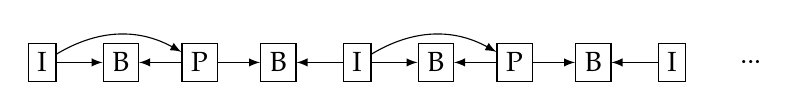
\begin{tikzpicture}[every path/.style={>=latex},every node/.style={draw,rectangle}]
\node            (a) at (0,0)  { I };
\node            (b) at (1,0)  { B };
\node            (c) at (2,0)  { P };
\node            (d) at (3,0)  { B };
\node            (e) at (4,0)  { I };
\node            (f) at (5,0)  { B };
\node            (g) at (6,0)  { P };
\node            (h) at (7,0)  { B };
\node            (i) at (8,0)  { I };
\node[draw=none]     at (9,0)  { ... };
\draw[->]            (a) edge (b);
\draw[->]            (c) edge (b);
\draw[->, bend left] (a) edge (c);
\draw[->]            (c) edge (d);
\draw[->]            (e) edge (d);
\draw[->]            (e) edge (f);
\draw[->]            (g) edge (f);
\draw[->, bend left] (e) edge (g);
\draw[->]            (g) edge (h);
\draw[->]            (i) edge (h);
\end{tikzpicture}
\end{center}
\caption{
A typical inter-coding structure with GOP size 4. \\
Arrows point from the reference to the dependent picture.
}
\label{fig:inter}
\end{figure}

In dependent views, it is common for every picture to have at least one
inter-view reference and every picture but the first to additionally be
inter-coded (\cite{vet11}, \cite{kha13}, e.g.). An example is given in
figure \ref{fig:inter-view}. This allows the encoder to take advantage of both
spatial and temporal redundancies in a dependent view.

\begin{figure}[H]
\begin{center}
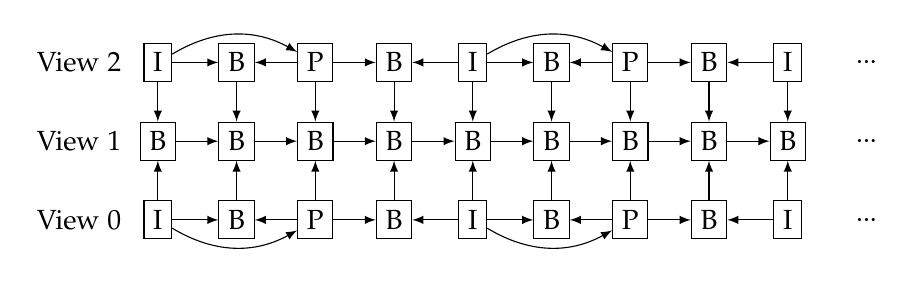
\begin{tikzpicture}[every path/.style={>=latex},every node/.style={draw,rectangle}]
\node[draw=none]      at (-1,0) { View 0 };
\node            (a0) at (0,0)  { I };
\node            (b0) at (1,0)  { B };
\node            (c0) at (2,0)  { P };
\node            (d0) at (3,0)  { B };
\node            (e0) at (4,0)  { I };
\node            (f0) at (5,0)  { B };
\node            (g0) at (6,0)  { P };
\node            (h0) at (7,0)  { B };
\node            (i0) at (8,0)  { I };
\node[draw=none]      at (9,0)  { ... };
\node[draw=none]      at (-1,1) { View 1 };
\node            (a1) at (0,1)  { B };
\node            (b1) at (1,1)  { B };
\node            (c1) at (2,1)  { B };
\node            (d1) at (3,1)  { B };
\node            (e1) at (4,1)  { B };
\node            (f1) at (5,1)  { B };
\node            (g1) at (6,1)  { B };
\node            (h1) at (7,1)  { B };
\node            (i1) at (8,1)  { B };
\node[draw=none]      at (9,1)  { ... };
\node[draw=none]      at (-1,2) { View 2 };
\node            (a2) at (0,2)  { I };
\node            (b2) at (1,2)  { B };
\node            (c2) at (2,2)  { P };
\node            (d2) at (3,2)  { B };
\node            (e2) at (4,2)  { I };
\node            (f2) at (5,2)  { B };
\node            (g2) at (6,2)  { P };
\node            (h2) at (7,2)  { B };
\node            (i2) at (8,2)  { I };
\node[draw=none]      at (9,2)  { ... };
\draw[->]             (a0) edge (b0);
\draw[->]             (c0) edge (b0);
\draw[->, bend right] (a0) edge (c0);
\draw[->]             (c0) edge (d0);
\draw[->]             (e0) edge (d0);
\draw[->]             (e0) edge (f0);
\draw[->]             (g0) edge (f0);
\draw[->, bend right] (e0) edge (g0);
\draw[->]             (g0) edge (h0);
\draw[->]             (i0) edge (h0);
\draw[->]             (a0) edge (a1);
\draw[->]             (b0) edge (b1);
\draw[->]             (c0) edge (c1);
\draw[->]             (d0) edge (d1);
\draw[->]             (e0) edge (e1);
\draw[->]             (f0) edge (f1);
\draw[->]             (g0) edge (g1);
\draw[->]             (h0) edge (h1);
\draw[->]             (i0) edge (i1);
\draw[->]             (a1) edge (b1);
\draw[->]             (b1) edge (c1);
\draw[->]             (c1) edge (d1);
\draw[->]             (d1) edge (e1);
\draw[->]             (e1) edge (f1);
\draw[->]             (f1) edge (g1);
\draw[->]             (g1) edge (h1);
\draw[->]             (h1) edge (i1);
\draw[->]             (a2) edge (a1);
\draw[->]             (b2) edge (b1);
\draw[->]             (c2) edge (c1);
\draw[->]             (d2) edge (d1);
\draw[->]             (e2) edge (e1);
\draw[->]             (f2) edge (f1);
\draw[->]             (g2) edge (g1);
\draw[->]             (h2) edge (h1);
\draw[->]             (i2) edge (i1);
\draw[->]             (a2) edge (b2);
\draw[->]             (c2) edge (b2);
\draw[->, bend left]  (a2) edge (c2);
\draw[->]             (c2) edge (d2);
\draw[->]             (e2) edge (d2);
\draw[->]             (e2) edge (f2);
\draw[->]             (g2) edge (f2);
\draw[->, bend left]  (e2) edge (g2);
\draw[->]             (g2) edge (h2);
\draw[->]             (i2) edge (h2);
\end{tikzpicture}
\end{center}
\caption{
A typical view-internal coding structure
with both dependent and reference pictures. \\
Pictures are both inter-coded and inter-view coded.
}
\label{fig:inter-view}
\end{figure}

In our tests, we chose to do away with the inter-coding in dependent views. We
did this for two reasons. First, the JMVC reference codec does not support
pictures that are both inter and inter-view coded in any configurable way.
Instead, it uses the same GOP structure for both dependent and reference views.
More importantly, however, doing away with inter-coding in the dependent views
allows us to isolate the coding efficiency achieved by inter-view coding alone,
without having to worry about the noise introduced by variable temporal
redundancy. From here on, we assume that all dependent and independent views
have internal structures as shown in figure \ref{fig:just-inter-view}.

\begin{figure}[H]
\begin{center}
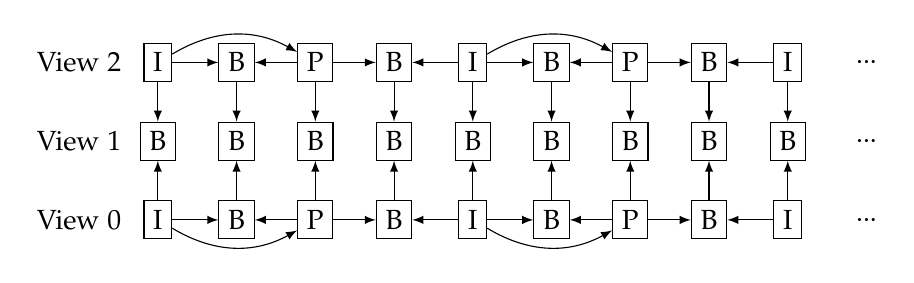
\begin{tikzpicture}[every path/.style={>=latex},every node/.style={draw,rectangle}]
\node[draw=none]      at (-1,0) { View 0 };
\node            (a0) at (0,0)  { I };
\node            (b0) at (1,0)  { B };
\node            (c0) at (2,0)  { P };
\node            (d0) at (3,0)  { B };
\node            (e0) at (4,0)  { I };
\node            (f0) at (5,0)  { B };
\node            (g0) at (6,0)  { P };
\node            (h0) at (7,0)  { B };
\node            (i0) at (8,0)  { I };
\node[draw=none]      at (9,0)  { ... };
\node[draw=none]      at (-1,1) { View 1 };
\node            (a1) at (0,1)  { B };
\node            (b1) at (1,1)  { B };
\node            (c1) at (2,1)  { B };
\node            (d1) at (3,1)  { B };
\node            (e1) at (4,1)  { B };
\node            (f1) at (5,1)  { B };
\node            (g1) at (6,1)  { B };
\node            (h1) at (7,1)  { B };
\node            (i1) at (8,1)  { B };
\node[draw=none]      at (9,1)  { ... };
\node[draw=none]      at (-1,2) { View 2 };
\node            (a2) at (0,2)  { I };
\node            (b2) at (1,2)  { B };
\node            (c2) at (2,2)  { P };
\node            (d2) at (3,2)  { B };
\node            (e2) at (4,2)  { I };
\node            (f2) at (5,2)  { B };
\node            (g2) at (6,2)  { P };
\node            (h2) at (7,2)  { B };
\node            (i2) at (8,2)  { I };
\node[draw=none]      at (9,2)  { ... };
\draw[->]             (a0) edge (b0);
\draw[->]             (c0) edge (b0);
\draw[->, bend right] (a0) edge (c0);
\draw[->]             (c0) edge (d0);
\draw[->]             (e0) edge (d0);
\draw[->]             (e0) edge (f0);
\draw[->]             (g0) edge (f0);
\draw[->, bend right] (e0) edge (g0);
\draw[->]             (g0) edge (h0);
\draw[->]             (i0) edge (h0);
\draw[->]             (a0) edge (a1);
\draw[->]             (b0) edge (b1);
\draw[->]             (c0) edge (c1);
\draw[->]             (d0) edge (d1);
\draw[->]             (e0) edge (e1);
\draw[->]             (f0) edge (f1);
\draw[->]             (g0) edge (g1);
\draw[->]             (h0) edge (h1);
\draw[->]             (i0) edge (i1);
\draw[->]             (a2) edge (a1);
\draw[->]             (b2) edge (b1);
\draw[->]             (c2) edge (c1);
\draw[->]             (d2) edge (d1);
\draw[->]             (e2) edge (e1);
\draw[->]             (f2) edge (f1);
\draw[->]             (g2) edge (g1);
\draw[->]             (h2) edge (h1);
\draw[->]             (i2) edge (i1);
\draw[->]             (a2) edge (b2);
\draw[->]             (c2) edge (b2);
\draw[->, bend left]  (a2) edge (c2);
\draw[->]             (c2) edge (d2);
\draw[->]             (e2) edge (d2);
\draw[->]             (e2) edge (f2);
\draw[->]             (g2) edge (f2);
\draw[->, bend left]  (e2) edge (g2);
\draw[->]             (g2) edge (h2);
\draw[->]             (i2) edge (h2);
\end{tikzpicture}
\end{center}
\caption{
The view-internal structure we use in our tests. \\
Pictures in the dependent view use inter-view coding only.
}
\label{fig:just-inter-view}
\end{figure}

[TODO: talk about hierarchical vs. non-hierarchical?]

With the view-internal coding structure established, we can now turn our
attention to the inter-view coding structure. There is little consensus in
the literature about what inter-view structure is best [TODO: is this true?].
In section \ref{sec:results}, we propose some optimal frame structures as
adduced from the results of our experiments.

\section{Related Work} %%%%%%%%%%%%%%%%%%%%%%%%%%%%%%%%%%%%%%%%%%%%%%%%%%%%%%%%%
\label{sec:related} %%%%%%%%%%%%%%%%%%%%%%%%%%%%%%%%%%%%%%%%%%%%%%%%%%%%%%%%%%%%
[TODO: fill this in if we need it]

\section{Experimental Method} %%%%%%%%%%%%%%%%%%%%%%%%%%%%%%%%%%%%%%%%%%%%%%%%%%
\label{sec:method} %%%%%%%%%%%%%%%%%%%%%%%%%%%%%%%%%%%%%%%%%%%%%%%%%%%%%%%%%%%%%
In this section, we describe the methods we used to obtain our results.
Subsections \ref{subsec:jmvc} and \ref{subsec:modifications} talk about the JMVC
reference codec and the modifications we made to it in order to obtain the data
we needed. In the process of performing those modifications, we identified a bug
in the codec, which we describe in subsection \ref{subsec:bug}. Finally, in
subsections \ref{subsec:data-set} and \ref{subsec:environment}, we talk about
the data sets we used and the hardware and software platform we ran our tests
on.

\subsection{Codec: JMVC}
\label{subsec:jmvc}
JMVC is the H.264 MVC reference codec \ref[sch10]. It is heavily adapted from
JM \ref{sue15}, the MPEG4/H.264 AVC reference codec. It contains a complete
implementation of the H.264 multiview extensions.

JMVC provides two methods of motion vector search: *block search*, which tests
every block in a region around the block being predicted for, and *TZ-search*,
which uses a combination of scaled-down raster search and diamond refinement
\cite{pur12}. We ran tests using both algorithms, but we will focus on our
results using TZ-search, since this most closely matches the way the codec would
be used in practice.

The codec also has several options when it comes to measuring the similarity
between blocks for motion compensation: sum of absolute differences (SAD); sum
of squared errors (SSE); or Hadamard. We used SAD for our tests, since it is
the simplest to reason about.

\subsection{Our Modifications}
\label{subsec:modifications}
In order to gather data about the coding process, we made the following changes
to the JMVC software:

\begin{enumerate}
\item We instrumented the process of writing motion vectors to the byte-stream
by first writing the same information in human-readable format to a text file.
This allowed us to examine the motion vectors to codec produced and compare them
the motion vectors we expected.

\item We inserted a timer around the process of encoding each picture, which
allowed us to determine exactly what portion of its time JMVC was spending on
each picture type.

\item We added a parameter to the configuration file that allowed us to
vertically constrain the motion-vector search space by a configurable amount.
\end{enumerate}

\subsection{A Bug in JMVC}
\label{subsec:bug}
In the process of making and testing these changes to JMVC, we discovered what
appears to be a bug in how JMVC searches the reference picture for similar
blocks. JMVC allows the motion-vector search space to be limited to a square of
configurable size around the dependent block. In some cases, however, this
square goes off the edge of the picture and must be further restricted to end
at the picture's edges. In the case where the square went off the top or left
edge, JMVC did not properly constrain this square, resulting in the
motion-vector search going out of the bounds of the array the represented the
reference picture. The resulting garbage would occasionally yield a block that
the encoder found similar enough, resulting in motion vectors that referred to
blocks off the edge of the picture. We have reported this bug to the software's
maintainers.

\subsection{Data Set}
\label{subsec:data-set}
We ran our tests on a 3D-rendered data-set constructed specifically for testing
multi-view coding. We ran tests on two data sets: The first is a scene of a
bedroom, in which the cameras pan up and to the right across the room. The
second depicts a helicopter taking off. A frame from each data set is shown in
figure \ref{fig:data-set}. All our tests were run over 300 frames.

\begin{figure}[H]
\centering
\begin{subfigure}{.5\textwidth}
\centering
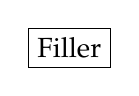
\begin{tikzpicture}[every path/.style={>=latex,bend left},every node/.style={draw,rectangle}] \node at (0,0) { Filler }; \end{tikzpicture}
%\includegraphics[scale=.5]{figures/bedroom1.png}
\caption{Bedroom}
\end{subfigure}%
\begin{subfigure}{.5\textwidth}
\centering
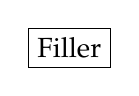
\begin{tikzpicture}[every path/.style={>=latex,bend left},every node/.style={draw,rectangle}] \node at (0,0) { Filler }; \end{tikzpicture}
%\includegraphics[scale=.5]{figures/helicopter.png}
\caption{Helicopter}
\end{subfigure}
\caption{A frame from each of the two data sets we used in our tests.}
\label{fig:data-set}
\end{figure}

Using constructed video streams, rather than the output of actual multiview
cameras allows us to avoid artifacts that might occur in real footage. For
example, the cameras might be slightly tilted or out of horizontal alignment,
or one of the cameras might have a flawed lens, decreasing the similarity
between views. Although these are considerations that come up in practice,
our interest is in gathering data about the common case, where the views
have the expected correlation.

\subsection{Testing Environment}
\label{subsec:environment}
All of our tests were performed on Red Hat Enterprise Linux using the SMP build
of kernel version 2.6.18-371.6.1.el5. We encoded the YUV files we used as input
to JMVC using ffmpeg version 0.6.5. Our times were collected using GNU Time
version 1.7 for the per-view encoding times and {\tt clock\_gettime()} using
Linux's {\tt CLOCK\_MONOTONIC}.

All our tests were performed on [TODO: zodiac cluster hardware information goes
here]

\section{Results} %%%%%%%%%%%%%%%%%%%%%%%%%%%%%%%%%%%%%%%%%%%%%%%%%%%%%%%%%%%%%%
\label{sec:results} %%%%%%%%%%%%%%%%%%%%%%%%%%%%%%%%%%%%%%%%%%%%%%%%%%%%%%%%%%%%
In this section, we present the results of our experiments and use them to make
judgements about how best to organize view dependencies, when to use
unidirectionally and bidirectionally coded views, and whether applying vertical
constraints to the motion-vector search of dependent views is worthwhile. The
former two points are discussed in subsection \ref{subsec:optimal}, while the
latter point is motivated and discussed in subsections
\ref{subsec:unconstrained} and \ref{subsec:constrained}, respectively.

\subsection{Finding the Optimal View Structure}
\label{subsec:optimal}
We knew from the outset that we wanted to test our constrained motion-vector
search under two scenarios. The first was the simple case of two adjacent views,
one depending on the other. This would let us determine the fundamental costs
and benefits of vertical constraints in a simple, idealized scenario. The view
structure that this scenario requires is obvious, and allows for no
optimization.

It is frequently desirable to encode more than two views, however, in order to
implement free-viewpoint video, for example, or in order to adjust the distance
of two stereoscopic views according to the user's proximity to the screen. To
model this scenario, we also wanted to perform tests using eight views. In this
case, however, it is far from obvious what the best choice of view structures
might be.

Since JMVC encodes at a variable bit-rate, there are two variables to optimize
for: bit-rate and time. In terms of time, the optimal configuration is to not
use motion compensation at all and make every view independent. This completely
fails to take advantage of spatial redundancies between views, however, and
presents only nominal bandwidth saving over simply having eight separate videos.

The optimal configuration in terms of bit-rate is harder to determine, since it
requires that we know how many bits, on average, each view type takes for each
possible distance from its reference view or views. We used our modified JMVC to
acquire this data. The bit-rates for single-reference pictures are presented in
figure \ref{fig:uniframes}, and the bit-rates for two-reference pictures are
given in figure \ref{fig:biframes}.

\begin{figure}
\centering
\includegraphics[width=.7\textwidth]{figures/motion_vector_data_unconstrained_unidirectional.pdf}
\caption{Average bit-rate for dependent view with one reference by distance
from the reference view.}
\label{fig:uniframes}
\end{figure}

\begin{figure}
\centering
\includegraphics[width=\textwidth]{figures/motion_vector_data_unconstrained_bidirectional.pdf}
\caption{Average bit-rate for dependent view with two references by distance
from the reference views.}
\label{fig:biframes}
\end{figure}

The first thing to notice is that the bit-rates in these figures are scaled to
percentage of the average independent view. This means that, in figure
\ref{fig:uniframes} for example, once the reference view is four views away,
it is no longer {\it ever} worthwhile to use single-reference motion
compensation in JMVC. It it is at least as cheap to encode the view
independently.

In figure \ref{fig:biframes}, it's clear that frames with two references scale
more efficiently to the distance of their reference frames. Perhaps
surprisingly, however, a bidirectionally coded view with a distance of one from
either of its references has at most a very slightly better bit-rate than a
unidirectional view with a distance of one from its reference. Since it is more
than twice as time-consuming, in the worst case, to use two references, this
implies that it is probably never profitable to use a dependent view with an
immediately adjacent references. Instead, bidirectional dependent views should
be used to compensate for being distant from potential references on both sides.

Based on this information, it seems that the optimal view configuration from the
perspective of bit-rate uses only single reference dependencies, as illustrated
in figure \ref{fig:hierarchical}. There is one more variable to consider,
however: It may be desirable to be able to split up the views and send just two
of them at a time for stereoscopic video. In this case, the hierarchical
dependencies in figure \ref{fig:hierarchical} would mean that in order to send
views 3 and 4, it would be necessary to send six views in total. Taking this
into consideration, we adopt the configuration in figure \ref{fig:optimal},
which takes up only slightly more space and would require that at most four
views be sent to send any two views.

\begin{figure}[H]
\begin{center}
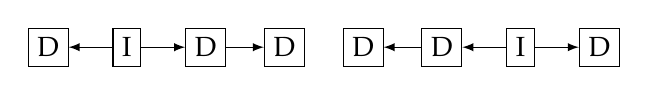
\begin{tikzpicture}[every path/.style={>=latex},every node/.style={draw,rectangle}]
\node            (a) at (0,0)  { D };
\node            (b) at (1,0)  { I };
\node            (c) at (2,0)  { D };
\node            (d) at (3,0)  { D };
\node            (e) at (4,0)  { D };
\node            (f) at (5,0)  { D };
\node            (g) at (6,0)  { I };
\node            (h) at (7,0)  { D };
\draw[->]             (b) edge (a);
\draw[->]             (b) edge (c);
\draw[->]             (c) edge (d);
\draw[->]             (g) edge (h);
\draw[->]             (g) edge (f);
\draw[->]             (f) edge (e);
\end{tikzpicture}
\end{center}
\caption{
Hierarchical configuration of \textbf{I}ndependent and \textbf{D}ependent views.
}
\label{fig:hierarchical}
\end{figure}

\begin{figure}[H]
\begin{center}
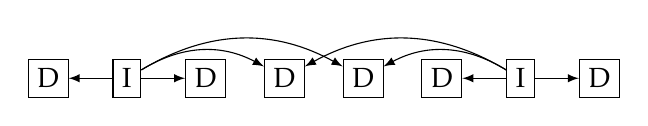
\begin{tikzpicture}[every path/.style={>=latex},every node/.style={draw,rectangle}]
\node            (a) at (0,0)  { D };
\node            (b) at (1,0)  { I };
\node            (c) at (2,0)  { D };
\node            (d) at (3,0)  { D };
\node            (e) at (4,0)  { D };
\node            (f) at (5,0)  { D };
\node            (g) at (6,0)  { I };
\node            (h) at (7,0)  { D };
\draw[->]             (b) edge (a);
\draw[->]             (b) edge (c);
\draw[->, bend left]  (b) edge (d);
\draw[->, bend right] (g) edge (d);
\draw[->]             (g) edge (h);
\draw[->]             (g) edge (f);
\draw[->, bend right] (g) edge (e);
\draw[->, bend left]  (b) edge (e);
\end{tikzpicture}
\end{center}
\caption{
Our optimal configuration of \textbf{I}ndependent and \textbf{D}ependent views.
}
\label{fig:optimal}
\end{figure}

\subsection{Distribution of Unconstrained Motion Vectors}
\label{subsec:unconstrained}

\subsection{Benefits of Vertical Constraint}
\label{subsec:constrained}

\section{Conclusion} %%%%%%%%%%%%%%%%%%%%%%%%%%%%%%%%%%%%%%%%%%%%%%%%%%%%%%%%%%%
\label{sec:conclusion} %%%%%%%%%%%%%%%%%%%%%%%%%%%%%%%%%%%%%%%%%%%%%%%%%%%%%%%%%
[TODO: add a conclusion]

\begin{thebibliography}{10} %%%%%%%%%%%%%%%%%%%%%%%%%%%%%%%%%%%%%%%%%%%%%%%%%%%%
\bibitem{sch10}
Schwarz, H.; Hinz, T.; Suehring, K.,
JMVC software model Version 8.2, May 2010

\bibitem{sue15}
Suehring, K., JM software model Version 19.0, May 2015

\bibitem{pur12}
Purnachand, N.; Alves, L.N.; Navarro, A.,
"Improvements to TZ search motion estimation algorithm for multiview video
coding," in Systems, Signals and Image Processing (IWSSIP),
pp.388--391, April 2012

\bibitem{vet11}
Vetro, A.; Wiegand, T.; Sullivan, G.J.,
"Overview of the Stereo and Multiview Video Coding Extensions of the
H.264/MPEG-4 AVC Standard," in Proceedings of the IEEE,
vol.99, no.4, pp.62-6-642, April 2011

\bibitem{kha13}
Khattak, S.; Hamzaoui, R.; Ahmad, S.; Frossard, P.,
"Fast Encoding Techniques for Multiview Video Coding,"
in {\it Signal Processing: Image Communication},
vol.28, no.6, pp.569--580, July 2013

\end{thebibliography}

\end{document}
